% Build: python build_assets.py; XeLaTeX twice with -output-directory=_build.
\documentclass[aspectratio=1610,11pt]{beamer}
\usepackage{fontspec}
\usepackage[russian]{babel}
\setsansfont{Arial}
\setmainfont{Arial}
\usefonttheme{professionalfonts}
\usepackage{amsmath,booktabs,tabularx,array,graphicx,tikz}
\usetikzlibrary{arrows.meta,positioning}
\definecolor{Ink}{HTML}{222222}
\definecolor{Accent}{HTML}{176B75}
\definecolor{Second}{HTML}{B84D56}
\definecolor{Quiet}{HTML}{666666}
\setbeamercolor{normal text}{fg=Ink,bg=white}
\setbeamercolor{frametitle}{fg=Ink,bg=white}
\setbeamercolor{structure}{fg=Accent}
\setbeamerfont{normal text}{size=\fontsize{11}{13}}
\setbeamerfont{frametitle}{size=\fontsize{17}{20},series=\bfseries}
\setbeamertemplate{navigation symbols}{}
\setbeamertemplate{footline}{}
\setbeamersize{text margin left=8mm,text margin right=8mm}
\setbeamertemplate{frametitle}{\vspace{2.5mm}\insertframetitle\par\vspace{1mm}}
\setbeamertemplate{itemize item}{\small\textbullet}
\setlength{\parskip}{.7mm}
\renewcommand{\fact}[2]{\par\textcolor{Accent}{\textbf{#1.}} #2\par}
\newcommand{\finding}[1]{\par\vspace{.5mm}\textbf{#1}\par}
\newcommand{\detail}[1]{{\fontsize{10}{12}\selectfont #1\par}}
\newcommand{\tights}{\setlength{\itemsep}{1.5mm}\setlength{\parsep}{0pt}\setlength{\parskip}{0pt}}
\newenvironment{datatable}{\par\begingroup\fontsize{10.5}{12.5}\selectfont\setlength{\tabcolsep}{4pt}\renewcommand{\arraystretch}{1.2}}{\par\endgroup}
\newcolumntype{L}[1]{>{\raggedright\arraybackslash}p{#1}}
\newcommand{\RowsBaseline}{%
Исходная DiT & 32 & 6.192 & 21.971 & 250.8 \\%
VQDM, без дообучения & 4.150 & 15.726 & 27.929 & 144.8 \\%
}
\newcommand{\OriginalFID}{6.192}
\newcommand{\BaselineFID}{15.726}
\newcommand{\RowsWindows}{%
Начало: переходы 1--10 & 3.83\% \\%
Середина: переходы 21--30 & 37.03\% \\%
Конец: переходы 41--50 & 1.46\% \\%
}
\newcommand{\RowsFamilies}{%
adaLN: время и класс & 33.33\% & 30.80\% \\%
Attention: связи участков & 22.22\% & 11.68\% \\%
MLP: обработка признаков & 44.44\% & 16.67\% \\%
}
\newcommand{\TemporalThreeGlobal}{15.536}
\newcommand{\TemporalThreeSplit}{15.663}
\newcommand{\TemporalFiveGlobal}{15.644}
\newcommand{\TemporalFiveSplit}{15.695}
\newcommand{\RowsLocal}{%
Локальный лосс, равные веса времени & 0.65\% & [-0.33; +2.01] \\%
Средние шаги: вес $\times2$ & 0.96\% & [+0.09; +2.23] \\%
Средние шаги: вес $\times4$ & 0.40\% & [-0.26; +1.00] \\%
Выходы трёх блоков, средние $\times4$ & 0.43\% & [-0.29; +1.22] \\%
Приоритет строк adaLN + средние $\times4$ & 0.16\% & [+0.03; +0.29] \\%
}
\newcommand{\RowsTemporal}{%
VQDM до обновлений & 4.1501 & 15.726 & 144.79 \\%
Один набор, 1000 обновлений & 4.1501 & 15.644 & 145.92 \\%
Пять наборов, по 200 обновлений & 4.2588 & 15.695 & 145.44 \\%
}
\newcommand{\RowsRecode}{%
Выходы 28 блоков & 2.026 & 2.481 \\%
Предсказание всей DiT & 1.734 & 2.373 \\%
Известный добавленный шум & 3.015 & 4.133 \\%
}
\newcommand{\RowsFresh}{%
Выходы 28 блоков & 2.026 & 2.158 \\%
Предсказание всей DiT & 1.734 & 2.185 \\%
Известный добавленный шум & 3.015 & 4.188 \\%
}
\newcommand{\RowsRecodePlain}{%
Выходы 28 блоков & 0.002026 & 0.002481 \\%
Предсказание всей DiT & 0.001734 & 0.002373 \\%
Известный добавленный шум & 0.003015 & 0.004133 \\%
}
\newcommand{\RowsFreshPlain}{%
Выходы 28 блоков & 0.002026 & 0.002158 \\%
Предсказание всей DiT & 0.001734 & 0.002185 \\%
Известный добавленный шум & 0.003015 & 0.004188 \\%
}
\newcommand{\RowsQuality}{%
Кодбуки, выход учителя & 11.045 & 40.424 & 215.2 & 0.7470 & 0.7523 \\%
+ масштабы строк & 11.050 & 40.438 & 215.3 & 0.7498 & 0.7524 \\%
+ собственные состояния & 11.146 & 40.181 & 212.8 & 0.7536 & 0.7412 \\%
DDPM-цель, шаг 100 & 13.390 & 40.707 & 180.1 & 0.7008 & 0.7671 \\%
DDPM-цель, шаг 500 & 14.350 & 42.906 & 172.9 & 0.6988 & 0.7620 \\%
+ мягкий выбор индексов & 24.376 & 45.845 & 100.6 & 0.6148 & 0.6932 \\%
}
\newcommand{\RowsPilot}{%
VQDM до обновлений & 0.136118 & --- \\%
Шум до CFG & 0.130247 & 4.31\% \\%
Выход после CFG, равные веса & 0.129780 & 4.66\% \\%
Выход после CFG, средние $\times4$ & 0.128446 & 5.64\% \\%
}
\newcommand{\KDStart}{1.1629}
\newcommand{\KDEnd}{1.0078}
\newcommand{\KDGain}{13.33\%}
\newcommand{\KDSeconds}{937}
\newcommand{\SoftChanged}{3.92\%}
\newcommand{\SoftErrorFactor}{5.70}
\newcommand{\FreshGain}{47.04\%}

\hypersetup{pdftitle={Как сохранить качество DiT при сжатии весов},pdfauthor={},
  pdfsubject={Постановка, ход и результаты экспериментов по векторной квантизации DiT},
  pdfcreator={XeLaTeX},colorlinks=true,urlcolor=Accent}

\begin{document}

% 01: research question, before technical terminology.
\begin{frame}[t]{Как сжать модель и не испортить изображения?}
  \fact{Дано}{DiT-XL/2 --- готовая нейросеть, создающая изображения
  $256\times256$ по заданному классу: например, «кошка» или «самолёт».}
  \fact{Проблема}{Сеть хранит сотни миллионов чисел --- \textbf{весов}.
  Чем точнее хранятся эти числа, тем больше памяти занимает модель.}
  \fact{Задача}{Заменить веса компактным представлением примерно по 4 бита
  вместо 32, сохранив поведение исходной сети. Это называется \textbf{квантизацией}.}
  \vspace{3mm}
  \textbf{Порядок исследования:}
  \begin{enumerate}\tights
    \item Перенести готовый метод сжатия VQDM на DiT и измерить потери.
    \item Найти, какие части генерации чувствительны к этим потерям.
    \item Проверить способы обучения сжатой модели и выбрать перспективный.
  \end{enumerate}
\end{frame}

% 02: the diffusion loop and the separate visualization experiment.
\begin{frame}[t]{Изображение получается не за один проход}
  \fact{Старт}{Создаётся случайный шум в компактном представлении изображения
  --- \textbf{латенте}. На вход также подаются класс и номер текущего шага.}
  \begin{center}
    \begin{tikzpicture}[>=Stealth,font=\fontsize{11}{13}\selectfont,
      box/.style={draw=Ink,minimum height=12mm,align=center,inner sep=2mm},node distance=5mm]
      \node[box] (z) {Текущий\\латент};
      \node[box,right=of z] (net) {Вся DiT\\предсказывает шум};
      \node[box,right=of net] (step) {Правило DDPM\\обновляет латент};
      \draw[->] (z)--(net); \draw[->] (net)--(step);
      \draw[->] (step.south)--++(0,-6mm)-|(z.south)
        node[pos=.35,below]{повторить 50 раз};
    \end{tikzpicture}
  \end{center}
  \fact{В конце}{Отдельная сеть VAE переводит итоговый латент в видимую картинку.}
  \detail{DDPM50 --- 50 переходов. Кроме последнего, добавляется новый случайный шум;
  его величину задаёт предсказанная дисперсия. DDIM с $\eta=0$ не добавляет новый шум.}
  \finding{Веса DiT одинаковы на всех 50 шагах. Меняются входной латент и время.}
  \detail{Для наглядной проверки сохранены состояния после 0, 10, 20, 25, 30, 40 и 50 переходов:
  от шумового состояния до изображения. Это визуализация, не оценка качества.}
\end{frame}

% 03: distinguish depth of one network call from diffusion time.
\begin{frame}[t]{Что находится внутри одного прохода DiT}
  Латент имеет размер $32\times32\times4$. Он делится на участки $2\times2$:
  получается 256 участков, каждый содержит 16 чисел.
  \begin{center}
    \begin{tikzpicture}[>=Stealth,font=\fontsize{11}{13}\selectfont,
      box/.style={draw=Ink,minimum height=12mm,align=center,inner sep=2mm},node distance=5mm]
      \node[box] (p) {256 участков\\входного латента};
      \node[box,right=of p] (b) {28 последовательных\\блоков обработки};
      \node[box,right=of b] (h) {Выходной слой:\\шум и дисперсия};
      \draw[->] (p)--(b); \draw[->] (b)--(h);
    \end{tikzpicture}
  \end{center}
  \begin{datatable}
    \begin{tabular*}{\textwidth}{@{\extracolsep{\fill}}lll@{}}
      \toprule
      В каждом блоке & Назначение & Веса\\
      \midrule
      2 матрицы attention & Связать разные участки картинки & 5.31 млн\\
      2 матрицы MLP & Преобразовать признаки участков & 10.62 млн\\
      1 матрица adaLN & Учесть время и класс & 7.96 млн\\
      \bottomrule
    \end{tabular*}
  \end{datatable}
  \finding{Сжаты все $28\times5=140$ матриц: 668.86 млн весов.}
  \detail{У 28 блоков разные веса. Входная и выходная проекции, представления времени/класса,
  смещения и VAE не сжимаются. Промежуточные данные сети тоже не квантуются.}
\end{frame}

% 04: concrete meaning of a codebook and a discrete index.
\begin{frame}[t]{VQDM: веса заменяются номерами}
  \fact{Кодбук}{Небольшая таблица заранее подобранных векторов.
  Здесь в каждом кодбуке 256 строк по восемь чисел.}
  \fact{Представление}{Восемь соседних весов заменяются суммой четырёх строк:
  по одной из каждого кодбука. Номер выбранной строки называется \textbf{индексом}.}
  \[
    \underbrace{(w_1,\ldots,w_8)}_{\text{восемь исходных весов}}
    \ \approx\ s\,\bigl( C_1[i_1]+C_2[i_2]+C_3[i_3]+C_4[i_4]\bigr).
  \]
  \detail{$C_1,\ldots,C_4$ --- кодбуки; $i_1,\ldots,i_4$ --- индексы; $s$ --- масштаб строки матрицы.}
  \fact{Экономия}{Вместо восьми 32-битных чисел хранятся четыре 8-битных индекса:
  4 бита на вес. С таблицами и несжатыми частями всей DiT получается \textbf{4.1501 бита}.}
  \finding{У каждой из 140 матриц свои четыре кодбука: всего 560.}
  \detail{В базовом варианте один и тот же набор применяется на всех временах генерации.
  Объём оценивается для упакованного представления, а не по размеру исследовательского файла.}
\end{frame}

% 05: calibration inputs and three distinct measurements.
\begin{frame}[t]{Как подобрать таблицы и проверить результат}
  \fact{Калибровка}{Исходная DiT генерирует 256 примеров по 50 шагов.
  Для каждого слоя собирается статистика его входов --- \textbf{активаций}.
  Статистика всех времён объединяется.}
  \fact{Обучение VQDM}{Кодбуки и индексы подбираются так, чтобы
  \textbf{выход отдельного сжатого слоя} был близок к выходу исходного слоя.
  Учитывается, какие входы реально встречаются, а не только величина весов.}
  \begin{datatable}
    \begin{tabularx}{\textwidth}{@{}lX@{}}
      \toprule
      Проверка & Что именно сравнивается\\
      \midrule
      Ошибка слоя & Два выхода одного слоя на одинаковом входе\\
      Ошибка всей DiT & Предсказания шума после всех 28 блоков на одинаковом входе\\
      Ошибка генерации & Итоговые латенты после двух отдельных цепочек из 50 переходов\\
      \bottomrule
    \end{tabularx}
  \end{datatable}
  \finding{Лучше приблизить отдельный слой ещё не означает получить лучшую картинку.}
\end{frame}

% 06: first baseline and a plain-language metric definition.
\begin{frame}[t]{Первый результат: сжатие портит качество}
  \fact{Дано}{Исходная DiT и её версия, сжатая VQDM, без дополнительного обучения.
  Обе генерируют по 10\,000 изображений в одинаковых условиях.}
  \begin{datatable}
    \begin{tabular*}{\textwidth}{@{\extracolsep{\fill}}lrr@{}}
      \toprule
      Модель & Бит на параметр & FID: меньше лучше\\
      \midrule
      Исходная DiT & 32 & \OriginalFID\\
      Сжатая VQDM & 4.1501 & \BaselineFID\\
      \bottomrule
    \end{tabular*}
  \end{datatable}
  \fact{Что такое FID}{Мера различия между наборами сгенерированных и реальных изображений.
  Это не процент ошибок; меньший FID означает более близкие распределения.}
  \fact{Получилось}{Расчётный объём весов уменьшился примерно в 7.7 раза,
  но FID вырос с 6.192 до 15.726. Простого переноса VQDM недостаточно.}
  \finding{Следующий вопрос: где возникают ошибки, которые сильнее всего мешают генерации?}
  \detail{Условия генерации: DDPM50, усиление класса CFG $=1.5$, один и тот же VAE.
  CFG объединяет ответы сети с заданным классом и без него.}
\end{frame}

% 07: causal diagnostic by restoring one time window.
\begin{frame}[t]{Опыт 1. Когда важнее точная модель?}
  \fact{Дано}{Сжатая VQDM, 50 переходов. Контроль --- исходная DiT
  с теми же случайными числами.}
  \fact{Сделано}{На десяти переходах вместо сжатой сети временно включается исходная.
  На остальных сорока остаётся VQDM. Проверены 1000 пар генераций.}
  \begin{datatable}
    \begin{tabular*}{\textwidth}{@{\extracolsep{\fill}}lr@{}}
      \toprule
      Где включена исходная DiT & Снижение конечной ошибки\\
      \midrule
      \RowsWindows
      \bottomrule
    \end{tabular*}
  \end{datatable}
  \detail{Конечная ошибка --- NMSE: сумма квадратов разницы итоговых латентов,
  делённая на сумму квадратов исходного латента. Меньше лучше; это не FID.}
  \finding{Из трёх проверенных окон важнее середина, а не конец генерации.}
  \detail{Обратная проверка: если оставить сжатую сеть только на десяти переходах,
  наибольшая ошибка тоже остаётся у среднего окна. Это диагностика, не компактный новый метод.}
\end{frame}

% 08: sensitive parameter families and output branches.
\begin{frame}[t]{Опыт 2. Какие части модели особенно важны?}
  \fact{Дано}{Та же VQDM. Вместо временного окна теперь во всех блоках
  возвращаются исходные веса одного типа слоёв. Остальные остаются сжатыми.}
  \begin{datatable}
    \begin{tabular*}{\textwidth}{@{\extracolsep{\fill}}lrr@{}}
      \toprule
      Какие веса возвращены & Возвращено весов & Снижение конечной ошибки\\
      \midrule
      \RowsFamilies
      \bottomrule
    \end{tabular*}
  \end{datatable}
  \fact{Получилось}{Особенно заметен эффект adaLN --- слоя, через который
  время и класс управляют блоком. Но восстановление трети весов увеличивает размер модели.}
  \fact{Дополнительная проверка}{На каждом вызове сети отдельно подменены её ответы:
  предсказанный шум или дисперсия. Возврат исходного шума почти устраняет расхождение;
  возврат одной дисперсии влияет намного слабее.}
  \finding{Возникли две идеи: уделить внимание времени/adaLN и точнее повторять шум исходной сети.}
\end{frame}

% 09: unsuccessful experiments, 1/4.
\begin{frame}[t]{Опыты 3--5. Улучшить отдельные слои}
  \fact{Идея}{Раз середина генерации и adaLN чувствительны, сильнее учитывать
  их при обучении кодбуков. Старт --- готовая VQDM; размер не меняется.}
  \begin{datatable}
    \begin{tabular*}{\textwidth}{@{\extracolsep{\fill}}lr@{}}
      \toprule
      Что дополнительно подгонялось & Снижение конечной ошибки\\
      \midrule
      Выходы слоёв, все времена равноправны & 0.65\%\\
      То же, средние времена важнее в 2 / 4 раза & 0.96\% / 0.40\%\\
      Выходы трёх целых блоков & 0.30--0.43\%\\
      Управляющие части adaLN, усиленная середина & 0.16\%\\
      \bottomrule
    \end{tabular*}
  \end{datatable}
  \fact{Проверка}{256 пар генераций. Две послойные схемы не приняли изменений после округления;
  дополнительный поиск индексов в трёх блоках дал лишь 0.09--0.70\%.}
  \finding{Сильного выигрыша нет. Преимущество усиленной середины над равномерным обучением не установлено.}
  \detail{Дополнительный эффект веса $\times2$ против равных весов: $+0.31\%$,
  95\%-й интервал от $-0.13\%$ до $+0.87\%$; он включает отсутствие улучшения.}
\end{frame}

% 10: unsuccessful experiments, 2/4.
\begin{frame}[t]{Опыт 6. Свои кодбуки каждому времени?}
  \fact{Идея и действие}{Разделить 50 переходов на окна и подстроить для каждого
  свои таблицы по входам из этого окна. Индексы общие; меняются значения кодбуков.}
  \begin{datatable}
    \begin{tabular*}{\textwidth}{@{\extracolsep{\fill}}lrr@{}}
      \toprule
      Проверка на 10\,000 изображений & Общий набор: FID & По окнам: FID\\
      \midrule
      3 окна: 30 / 10 / 10 переходов & \TemporalThreeGlobal & \TemporalThreeSplit\\
      5 окон: по 10 переходов & \TemporalFiveGlobal & \TemporalFiveSplit\\
      \bottomrule
    \end{tabular*}
  \end{datatable}
  \detail{Каждый оконный набор обучается 200 обновлений; общий --- 600 / 1000,
  то есть столько же, сколько все отдельные вместе. Меньший FID лучше.}
  \fact{Получилось}{У пяти наборов меньше локальная ошибка своего окна на 1.27--3.96\%,
  но FID не лучше общего набора. Дополнительные таблицы занимают 9.18 МБ.}
  \fact{Насколько они разные}{У трёх наборов относительное различие значений
  составляет 1.3--1.8\%: сами таблицы близки.}
  \finding{Разделение по времени пока не оправдало усложнение и дополнительную память.}
\end{frame}

% 11: the teacher objective, explained before its results.
\begin{frame}[t]{Идея: повторять ответ всей сети}
  \fact{Почему}{Ошибки слоёв влияют друг на друга. Идея: подгонять
  итоговое предсказание после \textbf{всех 28 блоков}.}
  \begin{center}
    \begin{tikzpicture}[>=Stealth,font=\fontsize{11}{13}\selectfont,
      box/.style={draw=Ink,align=center,inner sep=2mm,minimum height=11mm}]
      \node[box] (x) at (0,0) {Один и тот же\\латент, время, класс};
      \node[box] (fp) at (5.1,.9) {Исходная DiT: ответ-образец};
      \node[box] (q) at (5.1,-.9) {Сжатая DiT: обучаемый ответ};
      \draw[->] (x.east)--(fp.west); \draw[->] (x.east)--(q.west);
      \draw[<->,Accent,thick] (fp.south)--(q.north);
    \end{tikzpicture}
  \end{center}
  \fact{Что меняется}{Ошибка между ответами передаётся назад через сжатую сеть.
  Исправляются только числа в кодбуках. Индексы и исходная DiT заморожены.}
  \finding{Кодбуки учатся компенсировать совместные ошибки слоёв без увеличения модели.}
  \detail{Это дистилляция: обучение по ответам исходной сети-учителя.
  Градиент проходит через один вызов DiT, не через 50 переходов генерации.}
\end{frame}

% 12: first positive paired generation experiment.
\begin{frame}[t]{Опыт 7. Достаточно ли подстроить три блока?}
  \fact{Дано и действие}{Готовая VQDM. Подстроены только кодбуки 4-го, 15-го и 26-го
  блоков: 15 матриц, 200 шагов оптимизации. Ответ сравнивается после всей сети.}
  \begin{datatable}
    \begin{tabular*}{\textwidth}{@{\extracolsep{\fill}}lrr@{}}
      \toprule
      Какой ответ учителя повторялся & Конечная ошибка & Её снижение\\
      \midrule
      Без дополнительного обучения & 0.136118 & ---\\
      Обычное предсказание шума & 0.130247 & 4.31\%\\
      Предсказание с усилением класса (CFG) & 0.129780 & 4.66\%\\
      То же, середина важнее в 4 раза & 0.128446 & 5.64\%\\
      \bottomrule
    \end{tabular*}
  \end{datatable}
  \fact{Как проверено}{256 пар полных генераций с одинаковыми шумами внутри пары.
  Во всех трёх случаях ошибка ниже; 95\%-е интервалы снижения не включают ноль.}
  \finding{Обучение по ответу всей DiT повлияло не только на учебную ошибку, но и на генерацию.}
  \detail{Это снижение расстояния до исходного итогового латента, не FID.
  Преимущество усиленной середины над обычным CFG отдельно не подтверждено.}
\end{frame}

% 13: three training signals, a separate initialization.
\begin{frame}[t]{Опыт 8. Какую цель выбрать для обучения?}
  \fact{Дано}{Другая серия: кодбуки заново подобраны по весам, без полной подготовки VQDM.
  Обучаются 140 матриц; индексы фиксированы.}
  \fact{Сравнение}{Три цели: повторить промежуточные выходы 28 блоков;
  повторить шум исходной DiT; предсказать известный шум, добавленный к реальной картинке.}
  \begin{datatable}
    \begin{tabular*}{\textwidth}{@{\extracolsep{\fill}}lrr@{}}
      \toprule
      Обучающая цель & После 200 обновлений & После 1000\\
      \midrule
      \RowsFreshPlain
      \bottomrule
    \end{tabular*}
  \end{datatable}
  \detail{Во всех ячейках --- средний квадрат ошибки ответа относительно исходной DiT,
  на одинаковых 96 отложенных входах. Меньше лучше. До обучения: 0.003274.}
  \finding{Ответ всей сети дал наименьшую ошибку: снижение на 47.04\% к шагу 200.
  На шаге 1000 она снова выросла.}
  \detail{47.04\% --- результат этой инициализации, не готового VQDM и не FID.}
\end{frame}

% 14: unsuccessful experiments, 3/4.
\begin{frame}[t]{Опыт 9. Поможет ли ещё и менять индексы?}
  \fact{Мотивация}{Изменение кодбука меняет сам образец для многих групп весов.
  Изменение индекса позволяет отдельной группе выбрать другой образец.}
  \fact{Дано и действие}{Та же свежая инициализация и три цели предыдущего опыта.
  Раз в 25 обновлений проверяются редкие замены индексов; принимаются только
  замены, уменьшающие ошибку на учебном наборе.}
  \begin{datatable}
    \begin{tabular*}{\textwidth}{@{\extracolsep{\fill}}lrr@{}}
      \toprule
      Цель, проверка на шаге 200 & Только кодбуки & И замены индексов\\
      \midrule
      \RowsRecodePlain
      \bottomrule
    \end{tabular*}
  \end{datatable}
  \detail{Снова показана ошибка ответа на отложенных входах: меньше лучше. Размер модели одинаков.}
  \finding{В этой схеме замены ухудшили результат при всех трёх целях.}
  \detail{Это не полный перебор индексов: принято лишь 4--11 тысяч замен из 334 млн назначений.
  Полезность других способов выбора индексов этим опытом не исключена.}
\end{frame}

% 15: fitting the completed native quantization.
\begin{frame}[t]{Опыт 10. Обучить кодбуки всех матриц}
  \fact{Дано}{Теперь старт --- \textbf{готовая сжатая VQDM}, а не свежая инициализация.
  Исходная DiT остаётся учителем. Обучаются кодбуки всех 140 матриц.}
  \begin{enumerate}\tights
    \item Из 4000 изображений ImageNet получены латенты. К каждому добавляется
      шум одного из 1000 уровней, выбранного случайно.
    \item Один и тот же зашумлённый латент подаётся в исходную и сжатую DiT.
      Обучающая цель --- сблизить предсказания шума и, с весом 0.1, дисперсии.
    \item Выполнено 500 небольших обновлений кодбуков. Индексы, масштабы,
      смещения и остальные веса не меняются.
  \end{enumerate}
  \fact{Контроль}{1000 изображений отложены. Ошибка измеряется на 96 фиксированных
  входах: 16 примеров на каждом из шести времён. Эти входы не используются для обучения.}
  \finding{Это дополнительное обучение, но не рост модели: остаётся 4.1501 бита на параметр.}
\end{frame}

% 16: the main completed same-input improvement.
\begin{frame}[t]{Результат: сеть точнее повторяет исходную}
  \fact{Проверка}{На каждом контрольном входе сравнивается предсказанный шум
  после всей DiT. Чем ниже кривая, тем ближе ответ к исходной сети.}
  {\centering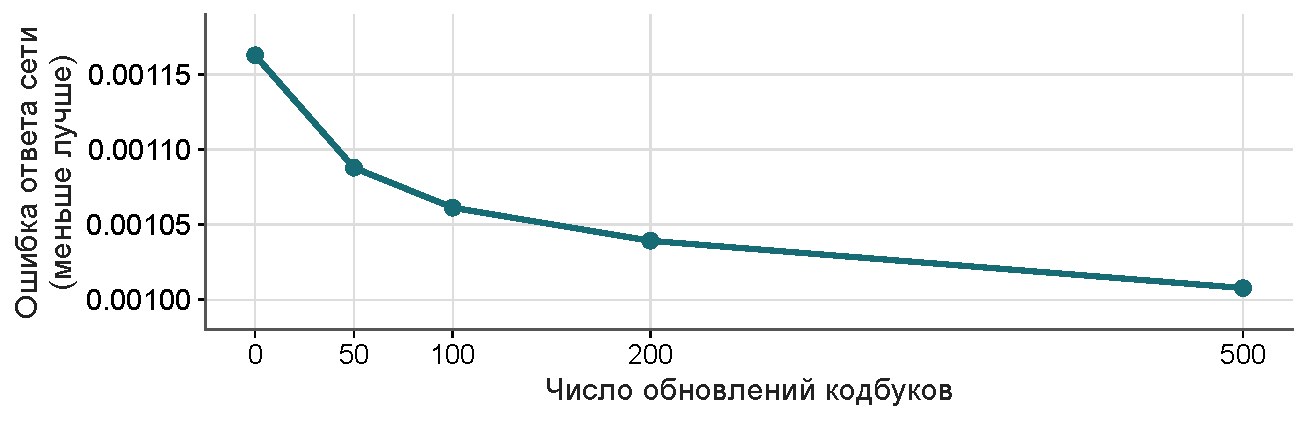
\includegraphics[width=.96\textwidth,height=37mm,keepaspectratio]{figures/native_learning.pdf}\par}
  \finding{Ошибка уменьшилась с 0.001163 до 0.001008: на 13.33\%.}
  \detail{Число шагов на графике --- обновления кодбуков, а не переходы генерации.
  Проверка проводится на отложенных входах. Это ещё не измерение улучшения картинок по FID.}
\end{frame}

% 17: unsuccessful experiments, 4/4.
\begin{frame}[t]{Опыты 11--14. Что добавить к этой подстройке?}
  \fact{Общие условия}{Все варианты начинают с одного готового VQDM;
  500 обновлений, одинаковая битность. Для оценки получены 5000 общих изображений.}
  \begin{datatable}
    \begin{tabularx}{\textwidth}{@{}L{.22\textwidth}Xr@{}}
      \toprule
      Вариант & Что изменено относительно простого обучения & FID $\downarrow$\\
      \midrule
      Контроль & Только кодбуки повторяют ответ исходной DiT & 11.045\\
      Масштабы & Дополнительно меняется величина строк весов & 11.050\\
      Свои входы & Половина входов взята из генераций сжатой сети & 11.146\\
      Известный шум & Вместо учителя --- шум и DDPM-цель дисперсии & 13.390\\
      Выбор индексов & Смесь двух строк кодбука при обучении; потом выбор одной & 24.376\\
      \bottomrule
    \end{tabularx}
  \end{datatable}
  \finding{Ни одно дополнение не улучшило FID относительно простого контроля.}
  \detail{Для DDPM показан лучший контрольный шаг 100; на шаге 500 FID = 14.350.
  У выбора индексов сменилось 3.92\% назначений, ошибка ответа выросла в 5.70 раза.
  Разницу 11.045 и 11.050 нельзя объявлять значимой без повторных обучений.}
\end{frame}

% 18: reproductions have no fabricated final metrics.
\begin{frame}[t]{Воспроизведение VQ4DiT и DPQ}
  \fact{Зачем}{Неудачная адаптация отдельной идеи не означает, что не работает
  метод статьи целиком. Нужны самостоятельные запуски авторских алгоритмов.}
  \begin{columns}[T,onlytextwidth]
    \begin{column}{.48\textwidth}
      \textbf{VQ4DiT}
      \par\textbf{Дано:} авторский код, DiT-XL/2.
      \par\textbf{Сделано:} свой кодбук у каждой матрицы;
      обучаются значения и выбор индексов. 500 обновлений.
      \par\textbf{Получилось:} обучение завершено, финальных метрик
      в сохранённом срезе нет.
    \end{column}
    \begin{column}{.48\textwidth}
      \textbf{DPQ}
      \par\textbf{Дано:} опубликованный код и описание статьи.
      \par\textbf{Сделано:} запущены опубликованный алгоритм и дополненная
      версия по описанию статьи. По одному проходу по обучающему ImageNet.
      \par\textbf{Получилось:} обучение завершено, генерация для метрик
      ещё не завершена в сохранённом срезе.
    \end{column}
  \end{columns}
  \finding{Совпадение с цифрами статей пока не установлено.}
  \detail{Это отдельные репродукции, не строки предыдущей таблицы. У DPQ оценка DDPM250;
  у VQ4DiT DDPM50 и другой VAE. Прямое сравнение без контроля условий некорректно.}
\end{frame}

% 19: evidence separated by what was measured.
\begin{frame}[t]{Что получилось установить}
  \begin{enumerate}\tights
    \item \textbf{Простого переноса VQDM недостаточно.}
      \par Веса занимают примерно в 7.7 раза меньше места,
      но FID вырос с 6.192 до 15.726 на 10\,000 изображений.
    \item \textbf{Чувствительность не равна готовому способу улучшения.}
      \par Середина генерации и adaLN важны, однако локальное усиление их роли
      и отдельные временные кодбуки не дали сильного выигрыша.
    \item \textbf{Перспективнее обучать по ответу всей исходной DiT.}
      \par На трёх блоках конечная ошибка генерации снизилась на 4.3--5.6\%.
      На всех кодбуках готового VQDM ошибка ответа сети снизилась на 13.33\%.
  \end{enumerate}
  \vspace{2mm}
  \finding{Это два разных положительных результата: ближе итоговый латент и точнее ответ сети.}
  \detail{Ни один из этих процентов не является снижением FID.
  Выводы относятся к проверенным настройкам; независимых повторов обучения пока нет.}
\end{frame}

% 20: the missing comparison and a concrete decision path.
\begin{frame}[t]{Что нужно, прежде чем заявлять улучшение}
  \fact{Не хватает одного контроля}{Новый FID 11.045 получен на 5000 изображений.
  Старый FID 15.726 --- на 10\,000. Разное число изображений влияет на FID,
  поэтому считать это доказанным улучшением нельзя.}
  \fact{Ближайшая проверка}{Завершить оценку VQDM \textbf{до подстройки}
  на тех же 5000 примерах и с теми же настройками, что после неё.
  Итоговых метрик этого контроля в сохранённом срезе ещё нет.}
  \fact{Если выигрыш подтвердится}{Провести независимые повторы обучения,
  проверить шаг обучения и момент остановки;
  затем провести общую более крупную оценку.}
  \fact{Параллельно}{Закончить метрики VQ4DiT и DPQ и сравнить с их статьями
  при совпадающих условиях генерации.}
  \finding{Рабочая гипотеза: качество лучше сохраняется, если кодбуки обучаются
  повторять поведение всей сети, а не только отдельных слоёв.}
\end{frame}

\end{document}
